% 原书印刷127--143／PDF物理152--168.
\subsection{Beckmann问题}\label{sec:4.2}

本节讨论Beckmann在20世纪50年代引入的一个流极小化问题\cite{b27}. 它是更广泛的一类凸优化问题的特殊情形，后者形如$\min\{\int H(\mathbf w)\,\mathrm dx:\nabla\cdot\mathbf w=\mu-\nu\}$，其中$H$为凸函数. 这里讨论$H(z)=|z|$的情形，它是Beckmann所研究成本类中的一个极限情形；事实上，Beckmann更关注严格凸成本. 严格凸性将在“讨论”部分的\autoref{sec:4.4.1}中考虑. 此处专注于线性成本，并花比一般情形更多篇幅讨论，是因为它与Monge问题等价. 我们将给出研究该等价性以及这一问题所需的全部工具.

\subsubsection{引言、形式等价与变体}\label{sec:4.2.1}

这里考虑Beckmann在20世纪50年代作为最优运输模型提出的问题的一个简单版本. Beckmann称其为\emph{连续运输模型}，当时并不知道Kantorovich的工作以及两个理论之间可能存在的联系.

\paragraph{Beckmann最小流问题}
\begin{problem}\label{obj:4.5}\index{N110@Neumann边界条件（Neumann conditions）|hyperpage}
考虑极小化问题
\begin{equation}\label{eq:4.4}
 (\mathrm{BP})\quad
 \min\left\{\int|\mathbf w(x)|\,\mathrm dx:
       \mathbf w:\Omega\to\mathbb R^d,\ \nabla\cdot\mathbf w=\mu-\nu\right\},
\end{equation}
其中散度条件应在弱意义下理解，并配以无通量边界条件，即对任意$\phi\in C^1(\overline\Omega)$，都有$-\int\nabla\phi\cdot\mathrm d\mathbf w=\int\phi\,\mathrm d(\mu-\nu)$.
\end{problem}

现在说明\hyperref[obj:4.5]{(BP)}与成本为$c(x,y)=|x-y|$的\hyperref[obj:1.2]{(KP)}之间确实存在等价性. 为此，考察下列论述与形式计算.

取问题\hyperref[obj:4.5]{(BP)}，将$\mathbf w$上的约束改写为
\begin{equation*}
\begin{aligned}
 &\sup_\phi\int_\Omega\nabla\phi\cdot\mathbf w\,\mathrm dx
                  +\int_\Omega\phi\,\mathrm d(\mu-\nu)\\
 &\qquad=\begin{cases}
 0,&\nabla\cdot\mathbf w=\mu-\nu,\\
 +\infty,&\text{其他情形}.
 \end{cases}
\end{aligned}
\end{equation*}
于是，可以将\hyperref[obj:4.5]{(BP)}写为
\begin{equation}\label{eq:4.5}
\begin{aligned}
 &\inf_{\mathbf w}\left(\int_\Omega|\mathbf w|\,\mathrm dx
      +\sup_\phi\int_\Omega\nabla\phi\cdot\mathbf w\,\mathrm dx
      +\int_\Omega\phi\,\mathrm d(\mu-\nu)\right)\\
 &\quad=\sup_\phi\left(\int_\Omega\phi\,\mathrm d(\mu-\nu)
       +\inf_{\mathbf w}\int_\Omega
                (|\mathbf w|-\nabla\phi\cdot\mathbf w)\,\mathrm dx\right),
\end{aligned}
\end{equation}
这里如同\autoref{sec:1}的计算一样，形式地交换了inf和sup. 然后注意到
\[
 \inf_{\mathbf w}\int_\Omega(|\mathbf w|-\nabla\phi\cdot\mathbf w)\,\mathrm dx
 =\begin{cases}
 0,&|\nabla\phi|\leq1,\\
 -\infty,&\text{其他情形}.
 \end{cases}
\]
由此得到\hyperref[obj:4.5]{(BP)}的对偶表述：
\[
 \sup\left\{\int_\Omega\phi\,\mathrm d(\mu-\nu):|\nabla\phi|\leq1\right\}.
\]
由于该问题恰好与\hyperref[obj:1.9]{(DP)}相同（这是因为$\operatorname{Lip}_1$函数恰好就是梯度不超过1的函数），便得到\hyperref[obj:4.5]{(BP)}与\hyperref[obj:1.2]{(KP)}的形式等价性. 称其只是形式上的，是因为尚未证明\eqref{eq:4.5}中的等号. 注意，还需要假设$\Omega$凸；否则，梯度不超过1的函数，只是关于$\Omega$内的测地距离为$\operatorname{Lip}_1$的函数.

上述大部分讨论，特别是关于\hyperref[obj:4.5]{(BP)}的讨论，都特定于成本等于距离$|x-y|$的情形. 一般而言，对形如$h(x-y)$的成本，若希望类似结果成立，$h$就需要是1次齐次的. 文献\cite{b195,b196}给出了一种将凸成本变成凸1次齐次成本的一般方法：增加一个对应于时间的变量.\footnote{\phantomsection\label{idx:root4-p128-benamou-brenier}\index{B015@Benamou--Brenier方法（Benamou-Brenier）|hyperpage}这样，成本形如$|x-y|^p$的流极小化问题就变为所谓的Benamou--Brenier问题，我们将在\autoref{sec:5}和\autoref{sec:6}中讨论；但这里不沿这一类比进一步推论.} 一个有趣的推广仍保留Euclid距离情形的形式，它涉及由Riemann距离$k(x)$导出的成本$c$.

确切地说，考虑
\[
 \min\left\{\int k(x)|\mathbf w(x)|\,\mathrm dx:
                               \nabla\cdot\mathbf w=\mu-\nu\right\}.
\]
\phantomsection\label{idx:root4-p129-weighted-distance}\index{D044@距离成本（distance costs）|hyperpage}\index{W163@加权距离（weighted distances）|hyperpage}通过与满足$|\nabla u|\leq k$的函数$u$的对偶，它对应于
\[
 \min\left\{\int d_k(x,y)\,\mathrm d\gamma(x,y):
                                      \gamma\in\Pi(\mu,\nu)\right\},
\]
其中$d_k(x,y)=\inf_{\omega(0)=x,\,\omega(1)=y}L_k(\omega)$，$L_k(\omega):=\int_0^1k(\omega(t))|\omega'(t)|\,\mathrm dt$，是与Riemann度量$k$关联的距离.

当希望为运动的非均匀成本建模时，例如由地理障碍或地形格局导致的成本，上述推广是适用的. 但这类模型不总令人满意，例如在城市运输中，我们希望考虑度量$k$通常并非预先已知，而是依赖于交通分布本身. “讨论”部分的\autoref{sec:4.4.1}将展开这一方面，同时考察某种意义上与之“相反”的一个完全不同的问题（\autoref{sec:4.4.2}）：考虑的不再是质量集中受到惩罚的运输问题（由于交通拥挤），而是鼓励质量集中的问题，这是所谓的规模经济，即运输的质量越大，单位成本越便宜.

\subsubsection{构造Beckmann问题的极小解}\label{sec:4.2.2}

关于\hyperref[obj:4.5]{(BP)}，首先应注意，该问题先验地并不适定：可能不存在一个在散度约束下使$L^1$范数最小的$L^1$向量场. 想到变分法中证明存在性的直接方法，就容易理解这一点：取一个极小化序列$\mathbf w_n$，希望抽出收敛子序列. 若能这样做，由$\mathbf w_n\rightharpoonup\mathbf w$就容易证明$\mathbf w$仍满足$\nabla\cdot\mathbf w=\mu-\nu$，因为关系
\[
 -\int\nabla\phi\cdot\mathbf w_n\,\mathrm dx=\int\phi\,\mathrm d(\mu-\nu)
\]
可在$n\to\infty$时取极限. 然而，信息$\int|\mathbf w(x)|\,\mathrm dx\leq C$不足以抽出收敛序列，即使弱收敛也不够. 事实上，$L^1$空间非自反，不能保证有界序列存在弱收敛子序列. 与此相反，对偶空间具有这一性质（自反空间也如此，粗略地说，它们是其对偶空间的对偶）.

注意，Beckmann提出的严格凸版本更容易处理，我们将在\autoref{sec:4.4.1}回顾它：例如，若极小化$\int|\mathbf w|^2\,\mathrm dx$，就能使用$L^2$中的弱紧性，它比$L^1$中的紧性容易获得得多.

为避开这一困难，我们为\hyperref[obj:4.5]{(BP)}选择其自然框架，即向量测度框架.

\begin{sourcebox}{知识回顾：向量测度}\label{box:4.2}\index{V156@向量测度（vector measures）|hyperpage}
\begin{definition*}
集合$\Omega$上的有限向量测度$\lambda$，是给每个Borel子集$A\subset\Omega$赋一个值$\lambda(A)\in\mathbb R^d$的映射，并满足：对每个不交并$A=\bigcup_iA_i$（$i\neq j$时$A_i\cap A_j=\varnothing$），都有
\[
 \sum_i|\lambda(A_i)|<+\infty,\qquad
 \lambda(A)=\sum_i\lambda(A_i).
\]
\end{definition*}
用$\mathscr M^d(\Omega)$表示$\Omega$上的有限向量测度集合. 对这种测度，可通过
\begin{equation*}
\begin{aligned}
 |\lambda|(A):=\sup\biggl\{&\sum_i|\lambda(A_i)|:
        A=\bigcup_iA_i,\\
       &i\neq j\text{ 时 }A_i\cap A_j=\varnothing\biggr\}
\end{aligned}
\end{equation*}
关联一个正标量测度$|\lambda|\in\mathscr M_+(\Omega)$. 这一标量测度称为$\lambda$的\emph{全变差测度}. 注意，为简单起见，这里只考虑$\mathbb R^d$上的Euclid范数，并写成$|\lambda|$而非$\|\lambda\|$；后一个记号保留给全变差测度的总质量，见下文. 对其他范数，也可作同样定义.

若$|\xi|\in L^1(\Omega,|\lambda|)$，则Borel函数$\xi:\Omega\to\mathbb R^d$关于$\lambda$的积分有良好定义，记为$\int\xi\cdot\mathrm d\lambda$，可按$\sum_{i=1}^d\int\xi_i\,\mathrm d\lambda_i$计算，从而归结为标量函数关于标量测度的积分. 也可将它定义为分片常值函数积分的极限.

\emph{泛函分析事实.} 量$\|\lambda\|:=|\lambda|(\Omega)$是$\mathscr M^d(\Omega)$上的一个范数；通过对偶配对$(\xi,\lambda)\mapsto\int\xi\cdot\mathrm d\lambda$，这个赋范空间是$C_0(\Omega;\mathbb R^d)$的对偶，后者是在无穷远处消失的$\Omega$上连续函数空间. 由此得到一种$\overset{*}{\rightharpoonup}$收敛，在该收敛下，$\mathscr M^d(\Omega)$中的有界集紧. 与标量测度一样，用$\rightharpoonup$表示与$C_b$函数对偶的弱收敛.

下面的事实有助于澄清这一点.
\begin{proposition*}
对每个$\lambda\in\mathscr M^d(\Omega)$，都存在Borel函数$u:\Omega\to\mathbb R^d$，使$\lambda=u\cdot|\lambda|$，且$|u|=1$在$|\lambda|$-几乎处处成立. 特别地，$\int\xi\cdot\mathrm d\lambda=\int(\xi\cdot u)\,\mathrm d|\lambda|$.
\end{proposition*}
\begin{proof}[证明草图]
由$\lambda\ll|\lambda|$及Radon--Nikodym定理，得到函数$u$的存在性：每个满足$|\lambda|(A)=0$的集合$A$显然满足$\lambda(A)=0$. 为证明$|u|=1$，可考虑集合$\{|u|<1-\varepsilon\}$和$\{u\cdot e>a\}$，其中遍历所有使单位球$B_1$包含于$\{x\in\mathbb R^d:x\cdot e\leq a\}$的超平面；事实上，$B_1=\bigcap_{e,a}\{x\in\mathbb R^d:x\cdot e\leq a\}$，且可将交缩减为可数交. 这些集合必须是零测集，否则与$|\lambda|$的定义矛盾.
\end{proof}
\end{sourcebox}

有了这些定义，便可证明下述定理. 用$\mathscr M^d_{\mathrm{div}}$表示散度为标量测度的向量测度空间.

\begin{theorem}\label{obj:4.6}
假设$\Omega$是$\mathbb R^d$中的紧凸区域. 则问题
\[
 (\mathrm{BP})\quad
 \min\bigl\{|\mathbf w|(\Omega):
     \mathbf w\in\mathscr M^d_{\mathrm{div}}(\Omega),\quad
     \nabla\cdot\mathbf w=\mu-\nu\bigr\}
\]
有解，这里散度在弱意义下规定，即对每个$\phi\in C^1(\overline\Omega)$，要求$-\int\nabla\phi\cdot\mathrm d\mathbf w=\int\phi\,\mathrm d(\mu-\nu)$，其中也包含无通量边界条件. 此外，其最小值等于\hyperref[obj:1.2]{(KP)}的最小值，而且可以从\hyperref[obj:1.2]{(KP)}的一个解构造\hyperref[obj:4.5]{(BP)}的一个解. 因此，这两个问题等价.
\end{theorem}
\begin{proof}
首先要证明\hyperref[obj:4.5]{(BP)}与\hyperref[obj:1.2]{(KP)}的最小值相等. 先证明$\min\hyperref[obj:4.5]{(\mathrm{BP})}\geq\min\hyperref[obj:1.2]{(\mathrm{KP})}$. 为此，任取满足$|\nabla\phi|\leq1$的函数$\phi\in C^1$. 对任意满足$\nabla\cdot\mathbf w=\mu-\nu$的$\mathbf w$，有
\[
 |\mathbf w|(\Omega)=\int_\Omega1\,\mathrm d|\mathbf w|
 \geq\int_\Omega(-\nabla\phi)\cdot\mathrm d\mathbf w
 =\int_\Omega\phi\,\mathrm d(\mu-\nu).
\]
\phantomsection\label{idx:root4-p131-duality}\index{D046@对偶问题（dual problems）|hyperpage}若取一列$\operatorname{Lip}_1\cap C^1$函数，一致收敛到满足$\int_\Omega u\,\mathrm d(\mu-\nu)=\max\hyperref[obj:1.9]{(\mathrm{DP})}=\min\hyperref[obj:1.2]{(\mathrm{KP})}$的Kantorovich势$u$（例如，取卷积$\phi_k=\eta_k*u$），便对任意可行$\mathbf w$得到
\[
 \int_\Omega\mathrm d|\mathbf w|\geq\min\hyperref[obj:1.2]{(\mathrm{KP})},
\]
即$\min\hyperref[obj:4.5]{(\mathrm{BP})}\geq\min\hyperref[obj:1.2]{(\mathrm{KP})}$.

接下来同时证明反向不等式，并说明如何从\hyperref[obj:1.2]{(KP)}的一个最优$\gamma$构造最优$\mathbf w$.

事实上，构造这一散度约束问题的解的一种方法如下，见\cite{b70}：取一个最优运输方案$\gamma$，构造向量测度$\mathbf w_{[\gamma]}$，通过\footnote{选择$\mathbf w_{[\gamma]}$这一特殊记号，是为了与将在\autoref{sec:4.2.3}中引入的对象$\mathbf w_Q$相区别.}
\[
 \langle\mathbf w_{[\gamma]},\xi\rangle
 :=\int_{\Omega\times\Omega}\int_0^1
     \omega_{x,y}'(t)\cdot\xi(\omega_{x,y}(t))\,\mathrm dt\,\mathrm d\gamma(x,y)
\]
对每个$\xi\in C^0(\Omega;\mathbb R^d)$定义它. 这里$\omega_{x,y}$是线段$[x,y]$的一种参数化，显然在此需要$\Omega$的凸性. 尽管对本证明并非重要，我们仍固定恒速参数化，即$\omega_{x,y}(t)=(1-t)x+ty$.

不难验证，这一测度满足散度约束：若取$\xi=\nabla\phi$，则
\begin{equation*}
\begin{aligned}
 \int_0^1\omega_{x,y}'(t)\cdot\xi(\omega_{x,y}(t))\,\mathrm dt
 &=\int_0^1\frac{\mathrm d}{\mathrm dt}
                  \bigl(\phi(\omega_{x,y}(t))\,\mathrm dt\\
 &=\phi(y)-\phi(x),
\end{aligned}
\end{equation*}
因此$\langle\mathbf w_{[\gamma]},\nabla\phi\rangle=\int\phi\,\mathrm d(\nu-\mu)$，并且$\mathbf w_{[\gamma]}\in\mathscr M^d_{\mathrm{div}}(\Omega)$.

为估计其质量，可注意到$|\mathbf w_{[\gamma]}|\leq\sigma_\gamma$，其中标量测度$\sigma_\gamma$通过
\begin{equation*}
\begin{aligned}
 \langle\sigma_\gamma,\phi\rangle
 &:=\int_{\Omega\times\Omega}\int_0^1
       |\omega_{x,y}'(t)|\phi(\omega_{x,y}(t))\,\mathrm dt\,\mathrm d\gamma,\\
 &\hspace{5em}\text{对所有 }\phi\in C^0(\Omega;\mathbb R)
\end{aligned}
\end{equation*}
定义，称为\emph{运输密度}. 事实上，还可以说得更多：利用Kantorovich势$u$（见\autoref{sec:3}），可以写出\footnote{使用Kantorovich势$u$的梯度时需要注意：我们使用了\autoref{obj:3.6}的结果，它给出$u$在运输射线上的可微性.}
\[
 \omega_{x,y}'(t)=-|x-y|\frac{x-y}{|x-y|}
              =-|x-y|\nabla u(\omega_{x,y}(t)).
\]
这对每个$t\in(0,1)$和每个$x,y\in\operatorname{spt}(\gamma)$成立：当$x\neq y$时，$\omega_{x,y}(t)$位于运输射线$[x,y]$内部；而当$x=y$时，两个表达式都为零.

由此，对每个$\xi\in C^0(\Omega;\mathbb R^d)$有
\begin{equation*}
\begin{aligned}
 \langle\mathbf w_{[\gamma]},\xi\rangle
 &=\int_{\Omega\times\Omega}\int_0^1
    -|x-y|\nabla u(\omega_{x,y}(t))\cdot\xi(\omega_{x,y}(t))
                           \,\mathrm dt\,\mathrm d\gamma(x,y)\\
 &=-\int_0^1\mathrm dt\int_{\Omega\times\Omega}
    \nabla u(\omega_{x,y}(t))\cdot\xi(\omega_{x,y}(t))
                             |x-y|\,\mathrm d\gamma(x,y).
\end{aligned}
\end{equation*}
引入由$\pi_t(x,y)=\omega_{x,y}(t)=(1-t)x+ty$给出的函数$\pi_t:\Omega\times\Omega\to\Omega$，就得到
\[
 \langle\mathbf w_{[\gamma]},\xi\rangle
 =-\int_0^1\mathrm dt\int_\Omega\nabla u(z)\cdot\xi(z)
                           \,\mathrm d\bigl((\pi_t)_\#(c\cdot\gamma)\bigr),
\]
其中$c\cdot\gamma$是$\Omega\times\Omega$上关于$\gamma$具有密度$c(x,y)=|x-y|$的测度. 另一方面，同样的计算给出
\begin{equation}\label{eq:4.6}
 \langle\sigma_\gamma,\phi\rangle
 =\int_0^1\mathrm dt\int_\Omega\phi(z)
                       \,\mathrm d\bigl((\pi_t)_\#(c\cdot\gamma)\bigr),
\end{equation}
于是$\langle\mathbf w_{[\gamma]},\xi\rangle=\langle\sigma_\gamma,-\xi\cdot\nabla u\rangle$，即
\[
 \mathbf w_{[\gamma]}=-\nabla u\cdot\sigma_\gamma.
\]
这给出$\mathbf w_{[\gamma]}$关于$\sigma_\gamma$的密度，并确认$|\mathbf w_{[\gamma]}|\leq\sigma_\gamma$.

$\sigma_\gamma$的质量显然为
\begin{equation*}
\begin{aligned}
 \int_\Omega\mathrm d\sigma_\gamma
 &=\int_\Omega\int_0^1|\omega_{x,y}'(t)|\,\mathrm dt\,\mathrm d\gamma(x,y)\\
 &=\int_{\Omega\times\Omega}|x-y|\,\mathrm d\gamma(x,y)
  =\min\hyperref[obj:1.2]{(\mathrm{KP})}.
\end{aligned}
\end{equation*}
由证明的第一部分，其他任何$\mathbf w$都不可能比这更好，因此证明了$\mathbf w_{[\gamma]}$的最优性. 这也证明$\min\hyperref[obj:4.5]{(\mathrm{BP})}=\min\hyperref[obj:1.2]{(\mathrm{KP})}$.
\end{proof}

\paragraph{Monge--Kantorovich系统与运输密度}
\phantomsection\label{idx:root4-p133-transport-density}\index{T151@传输密度（transport density）|hyperpage}刚定义的标量测度$\sigma_\gamma$称为运输密度. 它在\cite{b159}与\cite{b70,b71}中因不同目的而被引入. 在\cite{b70,b71}中，它与某些形状优化问题相联系，本书不讨论这些问题. 另一方面，\cite{b159}使用它给出了成本为$|x-y|$的Monge问题的最早一批解之一. 重要事实是，测度$\sigma=\sigma_\gamma$与Kantorovich势$u$共同解所谓的Monge--Kantorovich系统
\begin{equation}\label{eq:4.7}\index{K083@Kantorovich势（Kantorovich potentials）|hyperpage}\index{M102@Monge--Kantorovich系统（Monge-Kantorovich system）|hyperpage}
 \begin{cases}
 \nabla\cdot(\sigma\nabla u)=\mu-\nu&\text{在 }\Omega\text{ 中},\\
 |\nabla u|\leq1&\text{在 }\Omega\text{ 中},\\
 |\nabla u|=1&\sigma\text{-几乎处处}.
 \end{cases}
\end{equation}
这一系统先验地只在形式意义下得到求解，因为当$\sigma\notin L^1$时，$L^\infty$函数$\nabla u$与测度$\sigma$的乘积没有意义. 为克服这一困难，有两种可能：使用$\sigma$-切向梯度理论（例如见\cite{b145,b71}），或者给出保证$\sigma_\gamma\in L^1$的条件. \autoref{sec:4.3}将采取第二条道路，并证明更好的$L^p$估计.

如前所述，\cite{b159}使用\eqref{eq:4.7}的解来寻找成本$|x-y|$的最优运输映射$\mathrm T$. 该映射定义为一个依赖于$\sigma$和$\nabla u$的向量场的流，恰好与\autoref{sec:4.2.3}将介绍的Dacorogna--Moser构造具有同样思想. 然而，由于$\sigma$和$\nabla u$缺少正则性，使用$p>1$时的问题$\min\{\int|\mathbf w|^p:\nabla\cdot\mathbf w=\mu-\nu\}$来逼近解为$\mathbf w=\sigma_\gamma\nabla u$的Beckmann问题$\min\{\int|\mathbf w|:\nabla\cdot\mathbf w=\mu-\nu\}$. 将在\autoref{sec:4.4.1}看到，这一与交通拥挤有关的问题由从某个$\Delta_{p'}$方程的解得到的向量场求解，并且具有一些正则性结果. 这样，Monge问题的对偶便由$p'\to\infty$时的$p'$-Laplace方程逼近.

\subsubsection{曲线测度的交通强度与交通流}\label{sec:4.2.3}\index{M098@曲线上的测度（measures on curves）|hyperpage}

本小节引入一些同时推广$\mathbf w_{[\gamma]}$与$\sigma_\gamma$的对象，它们有许多用途：既用于证明最优$\mathbf w$来自某个最优方案$\gamma$这一刻画，也用于“讨论”部分的建模问题. 作为副产品，还将给出Smirnov分解结果\cite{b287}的一个新证明，另见\cite{b278}.

\phantomsection\label{idx:root4-p134-ac-curves}\index{A008@绝对连续曲线（absolutely continuous curves）|hyperpage}先引入一些记号. 将$\mathrm{AC}(\Omega)$定义为绝对连续曲线$\omega:[0,1]\mapsto\Omega$的集合. 本节始终假设$\Omega$紧且有非空内部. 给定$\omega\in\mathrm{AC}(\Omega)$和连续函数$\phi$，令
\begin{equation}\label{eq:4.8}
 L_\phi(\omega):=\int_0^1\phi(\omega(t))|\omega'(t)|\,\mathrm dt.
\end{equation}
这一量是以$\phi$为权重的曲线长度. 取$\phi=1$，就得到$\omega$的通常长度，记为$L(\omega)$而非$L_1(\omega)$. 注意，这些量都有良好定义，因为$\omega\in\mathrm{AC}(\Omega)$蕴含$\omega$几乎处处可微，且$\omega'\in L^1([0,1])$. 回顾绝对连续曲线的定义：它们是分布导数$\omega'\in L^1$，并且对每个$t_0<t_1$都满足$\omega(t_1)-\omega(t_0)=\int_{t_0}^{t_1}\omega'(t)\,\mathrm dt$的曲线. 为简单起见，今后在区域不会产生歧义时，以$\mathscr C$（“曲线”空间）表示$\mathrm{AC}(\Omega)$.

考虑空间$\mathscr C$上的概率测度$Q$. 只讨论满足$\int L(\omega)\,\mathrm dQ(\omega)<+\infty$的测度；按照\cite{b48}引入的术语，这些测度称为\emph{交通方案}（traffic plans）. 在$\mathscr C$上采用一致收敛. 注意，Ascoli--Arzel\`a定理保证，对每个$\ell$，集合$\{\omega\in\mathscr C:\operatorname{Lip}(\omega)\leq\ell\}$关于一致收敛是紧的. 对这样的$Q$，将关联$\Omega$上的两个测度. 第一个是标量测度，称为\emph{交通强度}（traffic intensity），记为$i_Q\in\mathscr M_+(\Omega)$，对所有$\phi\in C(\Omega,\mathbb R_+)$通过
\begin{equation*}
\begin{aligned}
 \int_\Omega\phi\,\mathrm di_Q
 &:=\int_{\mathscr C}\left(\int_0^1\phi(\omega(t))|\omega'(t)|\,\mathrm dt\right)\mathrm dQ(\omega)\\
 &=\int_{\mathscr C}L_\phi(\omega)\,\mathrm dQ(\omega)
\end{aligned}
\end{equation*}
定义. 这一定义取自\cite{b112}，推广了运输密度的概念. 其解释如下：对一个子区域$A$，$i_Q(A)$表示$Q$在$A$中诱导的总累积交通，即对每条路径计算它在$A$中停留“多长”，然后在路径上取平均.

还通过
\begin{equation*}
\begin{aligned}
 &\int_\Omega\xi\cdot\mathrm d\mathbf w_Q
 :=\int_{\mathscr C}\left(\int_0^1\xi(\omega(t))\cdot\omega'(t)\,\mathrm dt\right)\mathrm dQ(\omega),\\
 &\hspace{5em}\forall\xi\in C(\Omega;\mathbb R^d)
\end{aligned}
\end{equation*}
为任意交通方案$Q\in\mathscr P(\mathscr C)$关联一个向量测度$\mathbf w_Q$. 将$\mathbf w_Q$称为$Q$诱导的\emph{交通流}（traffic flow）. 在上一定义中取梯度场$\xi=\nabla\phi$，得到
\begin{equation*}
\begin{aligned}
 \int_\Omega\nabla\phi\cdot\mathrm d\mathbf w_Q
 &=\int_{\mathscr C}[\phi(\omega(1))-\phi(\omega(0))]\,\mathrm dQ(\omega)\\
 &=\int_\Omega\phi\,\mathrm d\bigl((e_1)_\#Q-(e_0)_\#Q\bigr),
\end{aligned}
\end{equation*}
其中$e_t$表示时刻$t$的取值映射，即$e_t(\omega):=\omega(t)$.

从现在起，将注意力限制在\emph{可行交通方案}$Q$上，即满足$(e_0)_\#Q=\mu$、$(e_1)_\#Q=\nu$的交通方案，其中$\mu$和$\nu$是$\Omega$上给定的两个概率测度. 这意味着
\[
 \nabla\cdot\mathbf w_Q=\mu-\nu,
\]
所以$\mathbf w_Q$是连接$\mu$和$\nu$的可行流. 注意，散度始终在弱（分布）意义下考虑，并自动配有无通量条件；即称$\nabla\cdot\mathbf w=f$时，意指对所有$\phi\in C^1(\overline\Omega)$，有$\int\nabla\phi\cdot\mathrm d\mathbf w=-\int\phi\,\mathrm df$，不对测试函数$\phi$的边界行为加任何条件.

回到$\mathbf w_Q$，容易验证$|\mathbf w_Q|\leq i_Q$，其中$|\mathbf w_Q|$是向量测度$\mathbf w_Q$的全变差测度. 一般而言，这一不等式并非等式，因为$Q$中的曲线可能产生抵消：设想有不可忽略数量的曲线以相反方向经过同一点，使得$\mathbf w_Q=0$而$i_Q>0$.

我们需要交通强度和交通流的一些性质.

\begin{proposition}\label{obj:4.7}
$\mathbf w_Q$和$i_Q$都在重参数化下不变，即若$\mathrm T:\mathscr C\to\mathscr C$满足：对每个$\omega$，曲线$\mathrm T(\omega)$只是$\omega$的时间重参数化，则$\mathbf w_{\mathrm T_\#Q}=\mathbf w_Q$且$i_{\mathrm T_\#Q}=i_Q$.

对每个$Q$，总质量$i_Q(\Omega)$等于曲线在$Q$下的平均长度，即$\int_{\mathscr C}L(\omega)\,\mathrm dQ(\omega)=i_Q(\Omega)$. 特别地，由交通方案的定义，$\mathbf w_Q$和$i_Q$都是有限测度.

若$Q_n\rightharpoonup Q$且$i_{Q_n}\rightharpoonup i$，则$i\geq i_Q$.

若$Q_n\rightharpoonup Q$、$\mathbf w_{Q_n}\rightharpoonup\mathbf w$且$i_{Q_n}\rightharpoonup i$，则$\|\mathbf w-\mathbf w_Q\|\leq i(\Omega)-i_Q(\Omega)$. 特别地，若$Q_n\rightharpoonup Q$且$i_{Q_n}\rightharpoonup i_Q$，则$\mathbf w_{Q_n}\rightharpoonup\mathbf w_Q$.
\end{proposition}
\begin{proof}
重参数化不变性来自$L_\phi(\omega)$和$\int_0^1\xi(\omega(t))\cdot\omega'(t)\,\mathrm dt$的重参数化不变性.

在$i_Q$的定义中用函数1测试，就得到公式$\int_{\mathscr C}L(\omega)\,\mathrm dQ(\omega)=i_Q(\Omega)$.

为验证$i\geq i_Q$，固定一个正测试函数$\phi\in C(\Omega)$，并假设$\phi\geq\varepsilon_0>0$. 写成
\begin{equation}\label{eq:4.9}
 \int_\Omega\phi\,\mathrm di_{Q_n}
 =\int_{\mathscr C}\left(\int_0^1\phi(\omega(t))|\omega'(t)|\,\mathrm dt\right)\mathrm dQ_n(\omega).
\end{equation}
注意，函数$\mathscr C\ni\omega\mapsto L_\phi(\omega)=\int_0^1\phi(\omega(t))|\omega'(t)|\,\mathrm dt$为正且关于$\omega$下半连续. 确实，若取序列$\omega_n\to\omega$，由下界$\phi\geq\varepsilon_0>0$，可假设$\int|\omega_n'(t)|\,\mathrm dt$有界. 于是可推出$\omega_n'\rightharpoonup\omega'$弱收敛（作为测度，或在$L^1$中），从而在抽取子序列后，存在测度$f\in\mathscr M_+([0,1])$使$f\geq|\omega'|$且$|\omega_n'|\rightharpoonup f$. 此外，$\phi(\omega_n(t))\to\phi(\omega(t))$一致收敛，故
\[
 \int\phi(\omega_n(t))|\omega_n'(t)|\,\mathrm dt
 \to\int\phi(\omega(t))\,\mathrm df(t)
 \geq\int\phi(\omega(t))|\omega'(t)|\,\mathrm dt.
\]
由此可在\eqref{eq:4.9}中取极限，得到
\begin{equation*}
\begin{aligned}
 \int\phi\,\mathrm di
 &=\lim_n\int\phi\,\mathrm di_{Q_n}
  =\liminf_n\int_{\mathscr C}L_\phi(\omega)\,\mathrm dQ_n(\omega)\\
 &\geq\int_{\mathscr C}L_\phi(\omega)\,\mathrm dQ(\omega)
  =\int\phi\,\mathrm di_Q.
\end{aligned}
\end{equation*}
若取任意测试函数$\phi$（没有下界），加上常数$\varepsilon_0$再应用前述论证，得到$\int(\phi+\varepsilon_0)\,\mathrm di\geq\int(\phi+\varepsilon_0)\,\mathrm di_Q$. 令$\varepsilon_0\to0$，由于$i$是有限测度且$\phi$任意，得到$i\geq i_Q$.

为验证最后一条性质，固定一个光滑向量测试函数$\xi$以及数$\lambda>1$，考察
\begin{equation}\label{eq:4.10}
\begin{aligned}
 \int_\Omega\xi\cdot\mathrm d\mathbf w_{Q_n}
 &=\int_{\mathscr C}\left(\int_0^1\xi(\omega(t))\cdot\omega'(t)\,\mathrm dt\right)\mathrm dQ_n(\omega)\\
 &=\int_{\mathscr C}\left(\int_0^1\xi(\omega(t))\cdot\omega'(t)\,\mathrm dt
                     +\lambda\|\xi\|_\infty L(\omega)\right)\mathrm dQ_n(\omega)\\
 &\quad-\lambda\|\xi\|_\infty i_{Q_n}(\Omega),
\end{aligned}
\end{equation}
这里仅仅加上再减去$i_{Q_n}$的总质量，而它等于$L(\omega)$在$Q_n$下的平均值. 现在注意，函数
\begin{equation*}
\begin{aligned}
 \mathscr C\ni\omega\mapsto&\int_0^1\xi(\omega(t))\cdot\omega'(t)\,\mathrm dt
                     +\lambda\|\xi\|_\infty L(\omega)\\
 &\qquad\geq(\lambda-1)\|\xi\|_\infty L(\omega)
\end{aligned}
\end{equation*}
关于$\omega$下半连续：使用与前面相同的论证，注意取$\omega_n\to\omega$时，可假设$L(\omega_n)$有界，并得到$\omega_n'\rightharpoonup\omega'$. 因此，在\eqref{eq:4.10}中取极限，得到
\begin{equation*}
\begin{aligned}
 \int_\Omega\xi\cdot\mathrm d\mathbf w
 &=\lim_n\int_\Omega\xi\cdot\mathrm d\mathbf w_{Q_n}\\
 &\geq\int_{\mathscr C}\left(\int_0^1\xi(\omega(t))\cdot\omega'(t)\,\mathrm dt
              +\lambda\|\xi\|_\infty L(\omega)\right)\mathrm dQ(\omega)
              -\lambda\|\xi\|_\infty i(\Omega)\\
 &=\int_\Omega\xi\cdot\mathrm d\mathbf w_Q
               +\lambda\|\xi\|_\infty(i_Q(\Omega)-i(\Omega)).
\end{aligned}
\end{equation*}
将$\xi$替换为$-\xi$，得到
\[
 \left|\int_\Omega\xi\cdot\mathrm d\mathbf w
             -\int_\Omega\xi\cdot\mathrm d\mathbf w_Q\right|
 \leq\lambda\|\xi\|_\infty(i(\Omega)-i_Q(\Omega)).
\]
令$\lambda\to1$，并对所有$\|\xi\|_\infty\leq1$的$\xi$取上确界，就得到所需估计$\|\mathbf w-\mathbf w_Q\|\leq i(\Omega)-i_Q(\Omega)$.

最后一条性质显然成立：事实上，可在抽取子序列后假设$\mathbf w_{Q_n}\rightharpoonup\mathbf w$对某个$\mathbf w$成立，而$i=i_Q$蕴含$\mathbf w=\mathbf w_Q$，这也蕴含整个序列收敛.
\end{proof}

\begin{sourcebox}{补充知识：Dacorogna--Moser运输}\label{box:4.3}\index{D037@Dacorogna--Moser方法（Dacorogna-Moser）|hyperpage}
这里给出\cite{b132}中思想的一个特殊情形，这些思想首次在\cite{b159}中用于最优运输.

\emph{构造.} 假设$\mathbf w:\Omega\to\mathbb R^d$是Lipschitz向量场，在$\partial\Omega$上满足$\mathbf w\cdot\mathbf n=0$，并且$\nabla\cdot\mathbf w=f_0-f_1$；其中$f_0,f_1$是正概率密度，为Lipschitz连续且有正下界. 于是可定义非自治向量场
\[
 \mathbf v_t(x)=\frac{\mathbf w(x)}{f_t(x)},\qquad
 f_t=(1-t)f_0+tf_1,
\]
并考虑Cauchy问题
\[
 \begin{cases}
 y_x'(t)=\mathbf v_t(y_x(t)),\\
 y_x(0)=x.
 \end{cases}
\]
为每个$x$关联由$y_x(\cdot)$给出的曲线$Y(x)$，以此定义映射$Y:\Omega\to\mathscr C$. 随后考察测度$Q=Y_\#f_0$以及$\varrho_t:=(e_t)_\#Q:=(Y_t)_\#f_0$. 由\autoref{sec:4.1.2}的讨论，$\varrho_t$解连续性方程$\partial_t\varrho_t+\nabla\cdot(\varrho_t\mathbf v_t)=0$. 另一方面，容易验证$f_t$也解同一方程，因为$\partial_tf_t=f_1-f_0$，且$\nabla\cdot(f_t\mathbf v_t)=\nabla\cdot\mathbf w=f_0-f_1$. 由\autoref{sec:4.1.2}的唯一性结果，从$\varrho_0=f_0$推出$\varrho_t=f_t$. 特别地，$x\mapsto y_x(1)$是从$f_0$到$f_1$的运输映射.
\end{sourcebox}

计算Dacorogna--Moser构造中测度$Q$对应的交通强度和交通流很有意思. 固定标量测试函数$\phi$：
\begin{equation*}
\begin{aligned}
 \int_\Omega\phi\,\mathrm di_Q
 &=\int_\Omega\int_0^1\phi(y_x(t))|\mathbf v_t(y_x(t))|
                                  \,\mathrm dt\,f_0(x)\,\mathrm dx\\
 &=\int_0^1\int_\Omega\varphi(y)|\mathbf v_t(y)|f_t(y)\,\mathrm dy\,\mathrm dt\\
 &=\int_\Omega\phi(y)|\mathbf w(y)|\,\mathrm dy,
\end{aligned}
\end{equation*}
所以$i_Q=|\mathbf w|$. 类似地，固定向量测试函数$\xi$，有
\begin{equation*}
\begin{aligned}
 \int_\Omega\xi\cdot\mathrm d\mathbf w_Q
 &=\int_\Omega\int_0^1\xi(y_x(t))\cdot\mathbf v_t(y_x(t))
                                  \,\mathrm dt\,f_0(x)\,\mathrm dx\\
 &=\int_0^1\int_\Omega\xi(y)\cdot\mathbf v_t(y)f_t(y)\,\mathrm dy\,\mathrm dt\\
 &=\int_\Omega\xi(y)\cdot\mathbf w(y)\,\mathrm dy,
\end{aligned}
\end{equation*}
这说明$\mathbf w_Q=\mathbf w$. 注意，此时有$|\mathbf w_Q|=i_Q$，这是因为在每个给定点，所有曲线都有相同方向，不可能发生抵消.

利用这些工具，我们希望证明Smirnov的一个分解结果\cite{b287}；为此还需要一个额外的逼近结果.

\begin{lemma}\label{obj:4.8}
考虑光滑紧区域$\Omega$上的两个概率$\mu,\nu\in\mathscr P(\Omega)$，以及在分布意义下满足$\nabla\cdot\mathbf w=\mu-\nu$并配有无通量边界条件的向量测度$\mathbf w\in\mathscr M^d_{\mathrm{div}}$. 则对每个将$\Omega$包含于其内部的光滑紧区域$\Omega'$，存在一族满足$\mathbf w^\varepsilon\cdot\mathbf n_{\Omega'}=0$的向量场$\mathbf w^\varepsilon\in C^\infty(\Omega')$，以及两族密度$\mu^\varepsilon,\nu^\varepsilon\in C^\infty(\Omega')$，它们有正常数下界$k_\varepsilon>0$，满足$\nabla\cdot\mathbf w^\varepsilon=\mu^\varepsilon-\nu^\varepsilon$和$\int_{\Omega'}\mu^\varepsilon=\int_{\Omega'}\nu^\varepsilon=1$，作为测度分别弱收敛至$\mathbf w,\mu,\nu$，并且满足$|\mathbf w^\varepsilon|\rightharpoonup|\mathbf w|$.
\end{lemma}
\begin{proof}
先将$\mu,\nu,\mathbf w$在$\Omega$外延拓为零，再与Gauss核$\eta_\varepsilon$在整个$\mathbb R^d$中卷积，得到$\widehat{\mathbf w}^\varepsilon:=\mathbf w*\eta_\varepsilon$、$\widehat\mu^\varepsilon:=\mu*\eta_\varepsilon$、$\widehat\nu^\varepsilon:=\nu*\eta_\varepsilon$，仍满足$\nabla\cdot\widehat{\mathbf w}^\varepsilon=\mu^\varepsilon-\nu^\varepsilon$. 由于Gauss核严格正，$\widehat\mu^\varepsilon$和$\widehat\nu^\varepsilon$的密度也严格正. 这些卷积后的密度和向量场本可以满足定理要求，但还必须处理支集（它不是$\Omega'$）和边界行为.

令$\int_{\Omega'}\widehat\mu^\varepsilon=1-a_\varepsilon$、$\int_{\Omega'}\widehat\nu^\varepsilon=1-b_\varepsilon$. 显然，$\varepsilon\to0$时$a_\varepsilon,b_\varepsilon\to0$. 还考虑$\widehat{\mathbf w}^\varepsilon\cdot\mathbf n_{\Omega'}$：由于$d(\Omega,\partial\Omega')>0$，且$\eta_\varepsilon$在原点以外局部一致趋于零，还有$|\widehat{\mathbf w}^\varepsilon\cdot\mathbf n_{\Omega'}|\leq c_\varepsilon$，其中$c_\varepsilon\to0$.

令$u^\varepsilon$为问题
\[
 \begin{cases}
 \Delta u^\varepsilon=\dfrac{a_\varepsilon-b_\varepsilon}{|\Omega'|}
           &\text{在 }\Omega'\text{ 内},\\[3pt]
 \dfrac{\partial u^\varepsilon}{\partial\mathbf n}
       =-\widehat{\mathbf w}^\varepsilon\cdot\mathbf n
           &\text{在 }\partial\Omega'\text{ 上},\\[3pt]
 \displaystyle\int_{\Omega'}u^\varepsilon=0
 \end{cases}
\]
的解，并令向量场$\delta^\varepsilon=\nabla u^\varepsilon$. 注意，由于$-\int_{\partial\Omega'}\widehat{\mathbf w}^\varepsilon\cdot\mathbf n_{\Omega'}=a_\varepsilon-b_\varepsilon$，解存在. 分部积分还给出
\begin{equation*}
\begin{aligned}
 \int_{\Omega'}|\nabla u^\varepsilon|^2
 &=-\int_{\partial\Omega'}u^\varepsilon
                  (\widehat{\mathbf w}^\varepsilon\cdot\mathbf n_{\Omega'})
   -\int_{\Omega'}u^\varepsilon\frac{a_\varepsilon-b_\varepsilon}{|\Omega'|}\\
 &\leq C\|\nabla u^\varepsilon\|_{L^2}(c_\varepsilon+a_\varepsilon+b_\varepsilon),
\end{aligned}
\end{equation*}
从而$\|\nabla u^\varepsilon\|_{L^2}\leq C(a_\varepsilon+b_\varepsilon+c_\varepsilon)\to0$. 这说明$\|\delta^\varepsilon\|_{L^2}\to0$.

现在取
\begin{equation*}
\begin{aligned}
 \mu^\varepsilon&=\widehat\mu^\varepsilon\restr\Omega'
                       +\frac{a_\varepsilon}{|\Omega'|},\\
 \nu^\varepsilon&=\widehat\nu^\varepsilon\restr\Omega'
                       +\frac{b_\varepsilon}{|\Omega'|},\\
 \mathbf w^\varepsilon&=\widehat{\mathbf w}^\varepsilon\restr\Omega'
                       +\delta^\varepsilon,
\end{aligned}
\end{equation*}
并验证所有要求均满足. 特别地，最后一条成立，是因为$\|\delta^\varepsilon\|_{L^1}\to0$，且由卷积的一般性质，$|\widehat{\mathbf w}^\varepsilon|\rightharpoonup|\mathbf w|$.
\end{proof}

\begin{remark}\label{obj:4.9}
若明确考虑对$\Omega'$的依赖，还可以对收敛至$\Omega$的一列区域$\Omega'_\varepsilon$（例如关于Hausdorff拓扑收敛）得到同样的陈述. 只需适当选择它们，使令$t_\varepsilon:=d(\Omega,\partial\Omega'_\varepsilon)$后，有$\|\eta_\varepsilon\|_{L^\infty(B(0,t_\varepsilon)^c)}\to0$. 对Gauss核，当$t_\varepsilon^2/\varepsilon\to\infty$时就满足这一条件；取$t_\varepsilon=\varepsilon^{1/3}$即可保证.
\end{remark}

有了这些工具，现在可以证明：
\begin{theorem}\label{obj:4.10}
对每个有限向量测度$\mathbf w\in\mathscr M^d_{\mathrm{div}}(\Omega)$及满足$\nabla\cdot\mathbf w=\mu-\nu$的$\mu,\nu\in\mathscr P(\Omega)$，存在交通方案$Q\in\mathscr P(\mathscr C)$，满足$(e_0)_\#Q=\mu$、$(e_1)_\#Q=\nu$，使得$|\mathbf w_Q|=i_Q\leq|\mathbf w|$，且
\[
 \|\mathbf w-\mathbf w_Q\|+\|\mathbf w_Q\|
 =\|\mathbf w-\mathbf w_Q\|+i_Q(\Omega)=\|\mathbf w\|.
\]
特别地，除非$\mathbf w_Q=\mathbf w$，否则$|\mathbf w_Q|\neq|\mathbf w|$.
\end{theorem}
\begin{proof}
由\autoref{obj:4.8}和\autoref{obj:4.9}，可以构造逼近序列$(\mathbf w^\varepsilon,\mu^\varepsilon,\nu^\varepsilon)\rightharpoonup(\mathbf w,\mu,\nu)$，其中各项为支于收敛至$\Omega$的区域$\Omega_\varepsilon$上的$C^\infty$函数. 对这一向量场序列应用Dacorogna--Moser构造，得到一列测度$Q_\varepsilon$. 可将它们视为$\mathscr C:=\mathrm{AC}(\Omega')$上的概率测度，其中$\Omega\subset\Omega_\varepsilon\subset\Omega'$，每个测度都集中于取值在$\Omega_\varepsilon$内的曲线. 它们满足$i_{Q_\varepsilon}=|\mathbf w^\varepsilon|$及$\mathbf w_{Q_\varepsilon}=\mathbf w^\varepsilon$. 可将$Q_\varepsilon$所支的曲线重新参数化为恒速曲线，不改变交通强度和交通流. 即使用满足$L(\omega)=\operatorname{Lip}(\omega)$的曲线. 等式
\begin{equation*}
\begin{aligned}
 \int_{\mathscr C}\operatorname{Lip}(\omega)\,\mathrm dQ_\varepsilon(\omega)
 &=\int_{\mathscr C}L(\omega)\,\mathrm dQ_\varepsilon(\omega)\\
 &=\int_{\Omega'}i_{Q_\varepsilon}
  =\int_{\Omega'}|\mathbf w^\varepsilon|\\
 &\to|\mathbf w|(\Omega')=|\mathbf w|(\Omega)
\end{aligned}
\end{equation*}
表明$\int_{\mathscr C}\operatorname{Lip}(\omega)\,\mathrm dQ_\varepsilon(\omega)$有界，因此$Q_\varepsilon$紧，因为集合$\{\omega\in\mathscr C:\operatorname{Lip}(\omega)\leq L\}$紧. 所以，抽取子序列后可假设$Q_\varepsilon\rightharpoonup Q$. 测度$Q$显然集中于取值在$\Omega$内的曲线. 构造时$Q_\varepsilon$满足$(e_0)_\#Q_\varepsilon=\mu^\varepsilon$和$(e_1)_\#Q_\varepsilon=\nu^\varepsilon$，故取极限得到$(e_0)_\#Q=\mu$和$(e_1)_\#Q=\nu$. 此外，由\autoref{obj:4.7}，因为$i_{Q_\varepsilon}=|\mathbf w_\varepsilon|\rightharpoonup|\mathbf v|$且$\mathbf w_{Q_\varepsilon}\rightharpoonup\mathbf w$，得到$|\mathbf w|\geq i_Q\geq|\mathbf w_Q|$和$\|\mathbf w-\mathbf w_Q\|\leq|\mathbf w|(\Omega)-i_Q(\Omega)$. 由此
\[
 \|\mathbf w-\mathbf w_Q\|+\|\mathbf w_Q\|
 \leq\|\mathbf w-\mathbf w_Q\|+i_Q(\Omega)\leq\|\mathbf w\|,
\]
而反向不等式$\|\mathbf w\|\leq\|\mathbf w-\mathbf w_Q\|+\|\mathbf w_Q\|$总是成立.
\end{proof}

\begin{remark}\label{obj:4.11}\index{C035@环（cycles）|hyperpage}
上述陈述包含\cite{b287}中定理C的一个较弱版本，即把任意$\mathbf w$分解为一个环流$\mathbf w-\mathbf w_Q$（称所有无散度向量测度为环流）以及由路径测度诱导的流$\mathbf w_Q$，并满足$\|\mathbf w\|=\|\mathbf w-\mathbf w_Q\|+\|\mathbf w_Q\|$. 与\cite{b287}中定理的唯一区别是，后者保证可选择集中于简单曲线的$Q$，而这里未考虑这一点；另一方面，\autoref{ex:27}给出了这一问题的部分解答.
\end{remark}

\begin{remark}\label{obj:4.12}
可以猜想在这一构造中一个环流会发生什么. 设想\autoref{fig:4.1}中的例子：$\Omega$由$\Omega^+$、$\Omega^-$两部分组成，$\operatorname{spt}(\mu)\cup\operatorname{spt}(\nu)\subset\Omega^+$，而$\mathbf w$的一个环流包含于$\Omega^-$中. 构造逼近$\mu^\varepsilon$和$\nu^\varepsilon$时，$\Omega^-$中将有正质量，但非常小. 由于$\mathbf v$定义中的分母，Dacorogna--Moser构造产生的曲线会非常快地沿该环流运动，多次经过环流中的每个点. 因此，$\Omega^-$中的流$\mathbf w^\varepsilon$由多次通过的很小质量产生. 这意味着，$\varepsilon\to0$时，这组曲线的测度$Q_\varepsilon$将在极限中消失. 所以，测度$Q$集中在始终位于$\Omega^+$内的曲线上，且$\Omega^-$上$\mathbf w_Q=0$. 然而，这样只是去掉了这个特定的环流；对于位于$\mu$和$\nu$具有正质量的区域中的环流，并不会发生同样的事. 特别地，不能保证$\mathbf w_Q$没有环流.
\end{remark}

\begin{figure}[htbp]
 \centering
 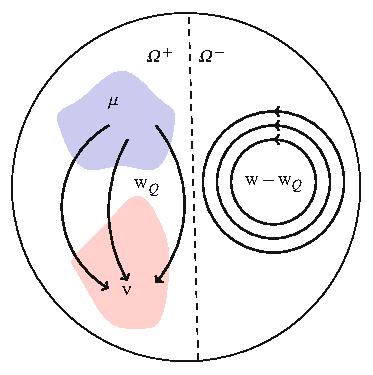
\includegraphics[width=.72\textwidth]{assets/ch04a-fig4-1.pdf}
 \caption{\autoref{obj:4.12}的例子中$\mathbf w$的分解.}
 \label{fig:4.1}
\end{figure}

\subsubsection{一维Beckman问题}\label{sec:4.2.4}

对于最优运输的Beckmann表述，一维情形非常简单，但仍值得分析：它既能检验与Monge表述的一致性，也能让我们在后续各节中使用这些结果. 取$\Omega=[a,b]\subset\mathbb R$.

首先注意，条件$\nabla\cdot\mathbf w=\mu-\nu$在一维中比高维中强得多. 事实上，散度是Jacobian矩阵的迹，因此指定散度，只是在一个先验具有$d\times d$个自由度的矩阵上施加一个约束. 与此相反，在一维中，向量场$\mathbf w$（实际上是标量）只有一个偏导数，这完全规定了$\mathbf w$的行为. 确实，条件$\nabla\cdot\mathbf w=\mu-\nu$配以Neumann边界条件，蕴含$\mathbf w$必为$\mu-\nu$的一个原函数，并满足$\mathbf w(a)=0$；$\mu$与$\nu$质量相同还蕴含$\mathbf w(b)=0$. 注意，导数是测度这一事实给出$\mathbf w\in BV([a,b])$；可以说，当$d=1$时，$\mathscr M^d_{\mathrm{div}}=BV$.

\Needspace{8\baselineskip}
\begin{sourcebox}{知识回顾：一元有界变差函数}\label{box:4.4}\index{B022@BV函数（BV functions）|hyperpage}
BV函数定义为分布导数是测度的$L^1$函数. 在一维中，这会带来许多结论. 特别地，这些函数几乎处处等于在逐点意义下全变差有界的函数：对每个$f:[a,b]\to\mathbb R$，定义
\begin{equation*}
\begin{aligned}
 TV(f;[a,b]):=\sup\biggl\{&\sum_{i=0}^{N-1}|f(t_{i+1})-f(t_i)|:\\
      &a=t_0<t_1<t_2<\cdots<t_N=b\biggr\}.
\end{aligned}
\end{equation*}
有界变差函数定义为满足$TV(f;[a,b])<\infty$的函数$f$. 容易验证，BV函数构成一个向量空间，且单调函数属于BV；事实上，若$f$单调，则$TV(f;[a,b])=|f(b)-f(a)|$. Lipschitz函数也属于BV，且$TV(f;[a,b])\leq\operatorname{Lip}(f)(b-a)$. 另一方面，连续函数不一定属于BV（但绝对连续函数属于BV），可微函数也不一定属于BV；当然，$C^1$函数在有界区间上为Lipschitz连续，因此属于BV. 例如，可以考虑
\[
 f(x)=\begin{cases}
 x^2\sin\left(\dfrac1{x^2}\right),&x\neq0,\\
 0,&x=0,
 \end{cases}
\]
它处处可微，却不属于BV.

另一方面，BV函数有若干性质.

\emph{$\mathbb R$中BV函数的性质.} 若$TV(f;[a,b])<\infty$，则$f$为两个单调函数之差；特别地，可以写成$f(x)=TV(f;[a,x])-(TV(f;[a,x])-f(x))$，两项都是非减函数. 它是有界函数，且$\sup f-\inf f\leq TV(f;[a,b])$；它与单调函数有相同的连续性和可微性性质：在每个点有左、右极限，除一个可数点集外连续，并且几乎处处可微.

特别地，一维中有$BV\subset L^\infty$，高维则并非如此；一般有$BV\subset L^{d/(d-1)}$.

最后强调与测度的联系：对$[a,b]$上的每个正测度$\mu$，取其累积分布函数$F_\mu(x)=\mu([a,x])$便可构造一个单调函数，且这一函数的分布导数恰为测度$\mu$. 反过来，紧区间上每个单调递增函数都是某个（唯一）正测度的累积分布函数，每个BV函数也都是某个（唯一）符号测度的累积分布函数.
\end{sourcebox}

由此得到下列事实：
\begin{itemize}
 \item 在一维中，只有一个竞争者$\mathbf w$，由$\mathbf w=F_\mu-F_\nu$给出，其中$F_\mu(x)=\mu([a,x])$、$F_\nu(x)=\nu([a,x])$.
 \item 这一场$\mathbf w$属于$BV([a,b])$，因此属于每个$L^p$空间，包括$L^\infty$.
 \item $\mathbf w$可能具有的更高正则性取决于$\mu-\nu$的正则性；例如，$\mu,\nu\in L^p$时，$\mathbf w\in W^{1,p}$.
 \item Beckmann问题的最小成本由$\|F_\mu-F_\nu\|_{L^1}$给出，这与\autoref{obj:2.17}一致.
 \item 由$\mathbf w=-u'\cdot\sigma$刻画的运输密度$\sigma$为$\sigma=|\mathbf w|$，并与$\mathbf w$有相同的可积性；它还是BV函数，因为它是BV函数与绝对值函数的复合.
\end{itemize}

\subsubsection[最优流的刻画与唯一性]{最优$\mathbf w$的刻画与唯一性}\label{sec:4.2.5}

本小节证明两个事实：首先，\hyperref[obj:4.5]{(BP)}中的最优$\mathbf w$总来自某个最优运输方案$\gamma$；然后，若两个测度之一绝对连续，所有最优$\gamma$都会给出相同的$\mathbf w_{[\gamma]}$以及相同的$\sigma_\gamma$.

\begin{theorem}\label{obj:4.13}
设$\mathbf w$在\hyperref[obj:4.5]{(BP)}中最优，则存在一个最优运输方案$\gamma$，使$\mathbf w=\mathbf w_{[\gamma]}$.
\end{theorem}
\begin{proof}
由\autoref{obj:4.10}，可以找到测度$Q\in\mathscr P(\mathscr C)$，满足$(e_0)_\#Q=\mu$、$(e_1)_\#Q=\nu$及$|\mathbf w|\geq|\mathbf w_Q|$. 然而，$\mathbf w$的最优性蕴含等式$|\mathbf w|=|\mathbf w_Q|$；由同一个\autoref{obj:4.10}，此时$\mathbf w=\mathbf w_Q$，并且$|\mathbf w|=i_Q$. 可假设$Q$集中于以恒速参数化的曲线上. 定义映射$S:\Omega\times\Omega\to\mathscr C$，为每个点对$(x,y)$关联恒速参数化的线段$\omega_{x,y}$，即$\omega_{x,y}(t)=(1-t)x+ty$. 只要证明$Q=S_\#\gamma$且$\gamma$为最优运输方案，就证明了陈述.

确实，再次利用$\mathbf w$的最优性和\autoref{obj:4.10}，得到
\begin{equation*}
\begin{aligned}
 \min\hyperref[obj:4.5]{(\mathrm{BP})}=|\mathbf w|(\Omega)=i_Q(\Omega)
 &=\int_{\mathscr C}L(\omega)\,\mathrm dQ(\omega)\\
 &\geq\int_{\mathscr C}|\omega(0)-\omega(1)|\,\mathrm dQ(\omega)\\
 &=\int_{\Omega\times\Omega}|x-y|\,\mathrm d\bigl((e_0,e_1)_\#Q\bigr)(x,y)\\
 &\geq\min\hyperref[obj:1.2]{(\mathrm{KP})}.
\end{aligned}
\end{equation*}
等式$\min\hyperref[obj:4.5]{(\mathrm{BP})}=\min\hyperref[obj:1.2]{(\mathrm{KP})}$蕴含这些不等式全为等式. 特别地，$Q$必须集中在满足$L(\omega)=|\omega(0)-\omega(1)|$的曲线上，也就是线段. 同时，属于$\Pi(\mu,\nu)$的测度$(e_0,e_1)_\#Q$必须在\hyperref[obj:1.2]{(KP)}中最优. 证明完毕.
\end{proof}

下一个结果的证明主要取自\cite{b8}.

\begin{theorem}\label{obj:4.14}
若$\mu\ll\mathscr L^d$，则向量场$\mathbf w_{[\gamma]}$不依赖于最优方案$\gamma$的选择.
\end{theorem}
\begin{proof}
固定$\mu$与$\nu$之间运输的一个Kantorovich势$u$. 这一势不依赖于$\gamma$的选择. 它确定了一个运输射线分划：\autoref{obj:3.8}保证，$\Omega$中同时属于多条运输射线的点，只可能是$u$的不可微点，因此是Lebesgue零测的. 用$S$表示属于多条运输射线的点集. 有$\mu(S)=0$，但不假设$\nu(S)=0$，因为$\nu$未假设绝对连续. 然而，$\gamma$集中于$(\pi_x)^{-1}(S^c)$. 因此可以按照包含点$x$的运输射线对$\gamma$作分解，见\autoref{sec:2.3}. 更精确地说，定义映射$R:\Omega\times\Omega\to\mathscr R$，取值于所有运输射线组成的集合$\mathscr R$，将每个点对$(x,y)$送至包含$x$的射线. 这在$\gamma$-几乎处处有良好定义，可写成$\gamma=\gamma^r\otimes\lambda$，其中$\lambda=R_\#\gamma$，并以$r$表示与运输射线相关的变量. 注意，对几乎每个$r\in\mathscr R$，方案$\gamma^r$在其自身的边缘之间最优；否则可以用一个最优方案将其替换，以可测的方式进行，便可降低$\gamma$的成本.

测度$\mathbf w_{[\gamma]}$也可通过这一分解得到，有$\mathbf w_{[\gamma]}=\mathbf w_{\gamma^r}\otimes\lambda$. 这意味着，为证明$\mathbf w_{[\gamma]}$不依赖于$\gamma$，只需证明每个$\mathbf w_{\gamma^r}$及测度$\lambda$不依赖于它. 对测度$\lambda$，这很容易：它是通过只依赖于$x$的映射得到的像测度，所以只依赖于$\mu$. 对$\mathbf w_{\gamma^r}$，注意，它是从一个最优方案$\gamma^r$按标准Beckmann方式得到的. 因此，由\autoref{sec:4.2.4}关于一维情形的讨论，它只由这一方案的边缘测度唯一确定.

所以，只需证明$(\pi_x)_\#\gamma^r$和$(\pi_y)_\#\gamma^r$不依赖于$\gamma$. 对$(\pi_x)_\#\gamma^r$仍然很容易，因为由分解的唯一性，它必定等于$\mu$关于映射$R$的分解. 对第二个边缘则更微妙.

将第二边缘$\nu^r:=(\pi_y)_\#\gamma^r$分解为两部分：
\[
 (\pi_y)_\#(\gamma^r\restr(\Omega\times S))
 +(\pi_y)_\#(\gamma^r\restr(\Omega\times S^c)).
\]
第二部分等于$\nu\restr S^c$的分解，它显然不依赖于$\gamma$，因为它只依赖于由$u$构造的集合$S$.

现在需要证明$\nu^r\restr S=(\pi_y)_\#(\gamma^r\restr(\Omega\times S))$不依赖于$\gamma$. 然而，这一测度只能集中于运输射线$r$的两个端点，因为不同运输射线只能在这些点相遇. 因此，这一测度是纯原子的，至多由两个Dirac质量组成. 不仅如此，$u$取得最大值的那个端点（即射线上次序的第一个点，见\autoref{sec:3.1}）不能含有任何$\nu$的质量. 事实上，运输必须在每条射线上沿指定方向进行，这是$\operatorname{spt}(\gamma)$上$u(x)-u(y)=|x-y|$的结果；要让目标测度在运输射线的“起点”处具有质量，唯一可能是源测度在该处也有原子. 然而，$\mu$绝对连续，并且性质N成立，见\autoref{sec:3.1.4}和\autoref{obj:3.12}，这意味着$\mu^r$具有原子的射线$r$构成的集合是零测集. 因此，$\nu^r\restr S$是单个Dirac质量. $\mu^r$与$\nu^r$的质量平衡条件蕴含，这一质量的值必定等于差$1-(\nu^r\restr S^c)(r)$；后一个量不依赖于$\gamma$，而只依赖于$\mu$和$\nu$.

最终，这证明了每个$\mathbf w_{\gamma^r}$都不依赖于$\gamma$的选择.
\end{proof}

\begin{corollary}\label{obj:4.15}
若$\mu\ll\mathscr L^d$，则\hyperref[obj:4.5]{(BP)}的解唯一.
\end{corollary}
\begin{proof}
\autoref{obj:4.13}已经证明，任意最优$\mathbf w$都形如$\mathbf w_{[\gamma]}$；而\autoref{obj:4.14}证明了所有场$\mathbf w_{[\gamma]}$都相同.
\end{proof}
